\videotitle{The Tree-Parzen Estimator (TPE)}

%-----------------------------------------------------------------------
\begin{frame}[c]{Overview of TPE \litw{\href{https://papers.nips.cc/paper/4443-algorithms-for-hyper-parameter-optimization.pdf}{Bergstra et al. 2011}}}

\begin{itemize}
    \item Standard Bayesian optimization models the probability $p(y \mid \conf)$ of observations $y$ given configurations $\conf$
    \item Instead, \alert{TPE fits kernel density estimators (KDEs) $l(\conf \mid y \le \gamma)$ and $g(\conf \mid y > \gamma)$}
    \myit{
        \item These KDEs are for ``good configurations'' (leading to objective function values below a threshold $\gamma$) and ``bad configurations''
        \item By default, $\gamma$ is set to the 15\% quantile of the observations
    }
    %\item \emph{Recall.} Bayesian optimization approach:
    %    \begin{equation*}
    %         P(\obs \vert \conf) \propto P(\conf \vert \obs) \times P(\obs)
    %    \end{equation*}
    %\item TPE then defines two such distributions, $l$ and $g$:
    %    \begin{equation*}
    %        P(\conf \vert \obs) = 
    %            \begin{cases}
    %                l(\conf) \text{ if } \obs < \obs^*\\
    %                g(\conf) \text{ otherwise} 
    %            \end{cases}
    %    \end{equation*}
    %where $\obs^*$ is an empirical threshold for a well-performing configuration (e.g., a $\gamma$ percentile of all observed $\obs$ in $D$).
    %\item Distributions are approximated by kernel density estimators (Parzen estimators)
\medskip
\fhpause
    \item Optimizing $l(\conf)/g(\conf)$ is equivalent to optimizing standard expected improvement in Bayesian optimization \lit{\href{https://papers.nips.cc/paper/4443-algorithms-for-hyper-parameter-optimization.pdf}{Bergstra et al. 2011}}
    
\medskip
\fhpause
    \item Why is the technique called TPE?
    \myit{
        \item The used KDEs are \alert{Parzen estimators}
        \item TPE can handle \alert{tree}-structured search spaces 
    }    
        
\end{itemize}


\end{frame}

%-----------------------------------------------------------------------
\begin{frame}[c]{TPE Example}

\onslide<1->
\begin{figure}
    \centering
    \only<1>{
        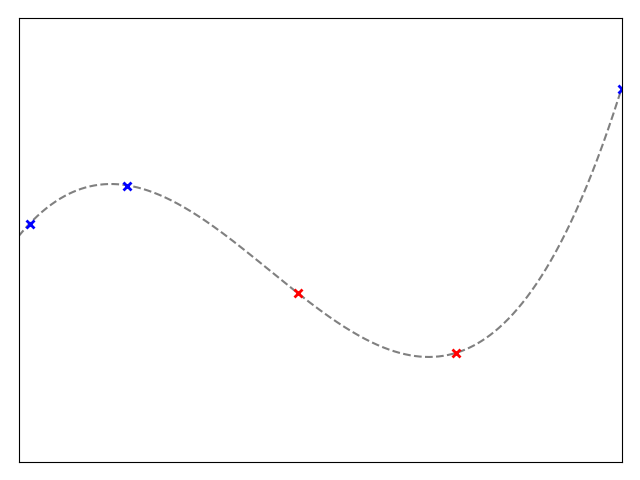
\includegraphics[width=0.6\textwidth]{images/tpe/tpeiter_1_observations.png}
    } \only<2>{
        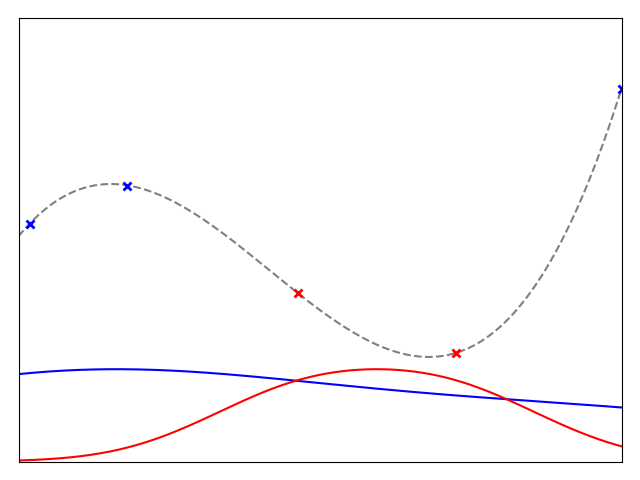
\includegraphics[width=0.6\textwidth]{images/tpe/tpeiter_1_pdfs.png}
    }\only<3>{
        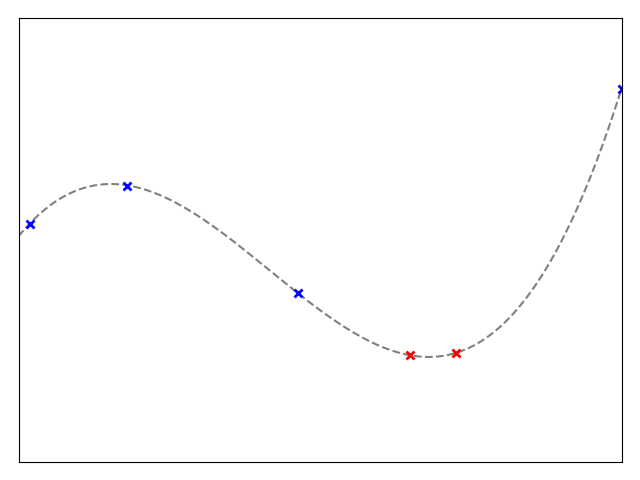
\includegraphics[width=0.6\textwidth]{images/tpe/tpeiter_2_observations.png}
    }\only<4>{
        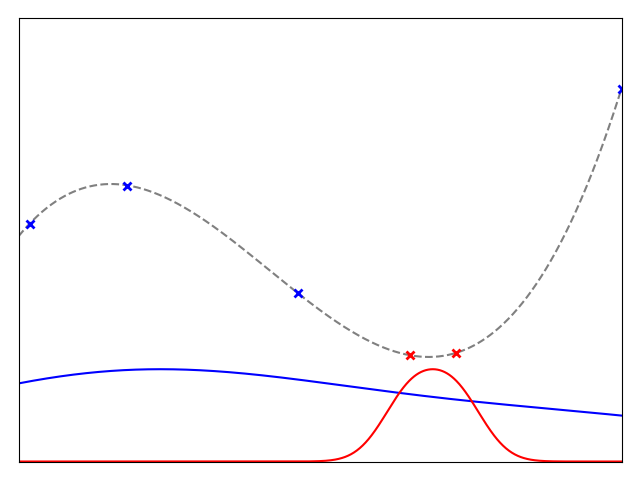
\includegraphics[width=0.6\textwidth]{images/tpe/tpeiter_2_pdfs.png}
    }\only<5>{
        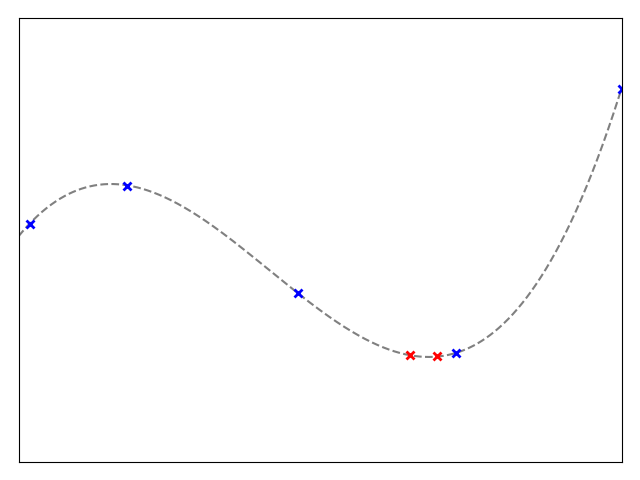
\includegraphics[width=0.6\textwidth]{images/tpe/tpeiter_3_observations.png}
    }\only<6>{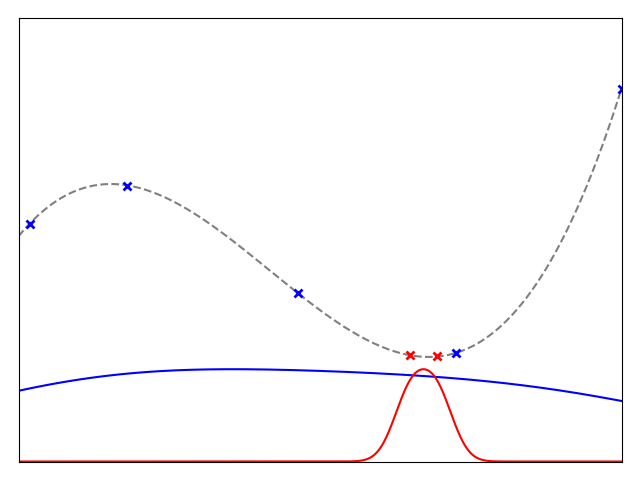
\includegraphics[width=0.6\textwidth]{images/tpe/tpeiter_3_pdfs.png}
    }
\end{figure}
\centering

\end{frame}
%-----------------------------------------------------------------------
%-----------------------------------------------------------------------
\begin{frame}[c]{TPE Pseudocode}


\begin{center}
\begin{minipage}{0.75\textwidth}
\begin{algorithm}[H]
    %\DontPrintSemicolon
    \SetAlgoLined
    \setcounter{AlgoLine}{0}
    \SetKwInOut{Require}{Require}
    \SetKwInOut{Result}{Result}
    \Require{Search space $\pcs$, 
    		cost function $\cost$, 
    		\textcolor{blue}{percentile $\gamma$},
    		maximal number of function evaluations $\bobudget$}
    \Result{Best observed configuration $\conf$ according to $\iter[\bobudget]{\dataset}$}
    
	Initialize data $\iter[0]{\dataset}$ with initial observations\;% \leftarrow \varnothing$\; 
    
    \For{$\bocount=1$ \KwTo $\bobudget$}{
		\textcolor{blue}{$\dataset_\text{good}, \dataset_\text{bad}$ $\leftarrow$ split $\iter[\bocount-1]{\dataset}$} according to quantile $\gamma$\

        \textcolor{blue}{$l(\conf)$, $g(\conf)$ $\leftarrow$ fit KDE on $\dataset_\text{good}$, $\dataset_\text{bad}$ respectively}\

		\textcolor{blue}{$\pcs_\text{cand}$ $\leftarrow$ draw samples from $l$};\

		\textcolor{blue}{Select next query point: $\bonextsample \in \argmax_{\conf \in \pcs_\text{cand}} l(\conf) / g(\conf)$}\
		
		Query $\bonextobs$\;
		
		$\iter[\bocount]{\dataset} \leftarrow \iter[\bocount-1]{\dataset} \cup \{\langle \bonextsample, \bonextobs \rangle \}$\;
	}
    \caption*{TPE loop}
\end{algorithm}
\end{minipage}
\end{center}


\end{frame}
%-----------------------------------------------------------------------

\begin{frame}[c]{Further Details}

Remarks:

\begin{itemize}
	\item TPE models $p(\conf | \obs)$
	\begin{itemize}
		\item we can multiply it with a prior to add expert knowledge
	\end{itemize}
	\smallskip
	
	\fhpause
	
	\item Performance of TPE depends on:
	\begin{itemize}
		\item setting of $\gamma$ to trade-off exploration and exploitation
		\item bandwidth of the KDEs 
	\end{itemize}
	
	\fhpause
	
	\smallskip
	
	\smallskip
	\item A successful tool implementing TPE is Hyperopt \lit{\href{https://github.com/hyperopt/hyperopt}{Bergstra et al.}}
\end{itemize}

\end{frame}
%-----------------------------------------------------------------------
\begin{frame}[c]{Summary}

\begin{columns}[T] % align columns
\begin{column}{.48\textwidth}
    \begin{block}{Advantages}
    \begin{itemize}
    	\item Computationally efficient: $O(Nd)$
    	\item Parallelizable
    	\item Robust
    	\item Can handle complex search spaces with priors
    \end{itemize}
    \end{block}
\end{column}%

\hfill%

\fhpause

\begin{column}{.48\textwidth}
    \begin{block}{Disadvantages}
    \begin{itemize}
    	\item Less sample-efficient than GPs
    \end{itemize}
    \end{block}
\end{column}
\end{columns}   

\end{frame}
%-----------------------------------------------------------------------
\begin{frame}[c]{Questions to Answer for Yourself / Discuss with Friends}

\begin{itemize}
    \item \alert{Disussion.} Is TPE really Bayesian optimization?
\medskip
    \item \alert{Disussion.} How does $\gamma$ impact the optimization procedure?
\medskip
    \item \alert{Derivation.} Go through the derivation that optimizing $l(\conf) / g(\conf)$ is equivalent to optimizing expected improvement; see Section 4.1 in \lit{\href{https://papers.nips.cc/paper/4443-algorithms-for-hyper-parameter-optimization.pdf}{Bergstra et al. 2011}}.
\end{itemize}

\end{frame}